\documentclass{ctexart}

\author{李约瀚 \\ 14130140331 \\ qinka@live.com \\ qinka@qinka.pw}
\title{FPGA 设计基础实验报告 (四)}

\usepackage{listings}
\lstset{breaklines}


\begin{document}


% Cover 
\thispagestyle{empty}
\begin{center}
  \vspace*{4em}
  {\Huge\textbf{FPGA设计基础实验报告\\\vspace*{0.5em} (三)}}
  \vfill
  \large
  \begin{tabular}{c@{:}l}
    班级 & 1413014 \\
    学号 & 14130140331 \\ 
    姓名 & 李约瀚 \\ 
    教师 & 沈沛意 \\
  \end{tabular} 
  \vspace*{4em}\\
\end{center}
\newpage

%% Settings
\setcounter{page}{0}
\setcounter{section}{0}

 % Exp 3-1

\section{Xilinx 嵌入式下系统设计(III)}
        
\subsection{实验目的}
\begin{itemize}
\item 了解 FPGA 嵌入式系统的设计基本概念与特点
\item 了解 MicroBlaze, 与对应的外设
\item 了解 EDK 开发的基本流程
\end{itemize}

\subsection{实验步骤}

\begin{itemize}
\item 自定义 IP 核
\item 自定义 IP 核逻辑
\item 添加 IP 核到硬件设计
\item 连接 IP 核
\item 生成网表与比特流
\item 生成软件工程
\item 添加自定义 IP 的驱动到 BSP
\item 上电上板
\end{itemize}


\subsection{实验内容}

\subsubsection{系统机构与设计}

系统完整的设计如图 \ref{fig:report3-1} 所示,其中本次实验的设计内容如图 \ref{fig:report4-1} 所示。
\begin{figure}[h!]
  \centering
  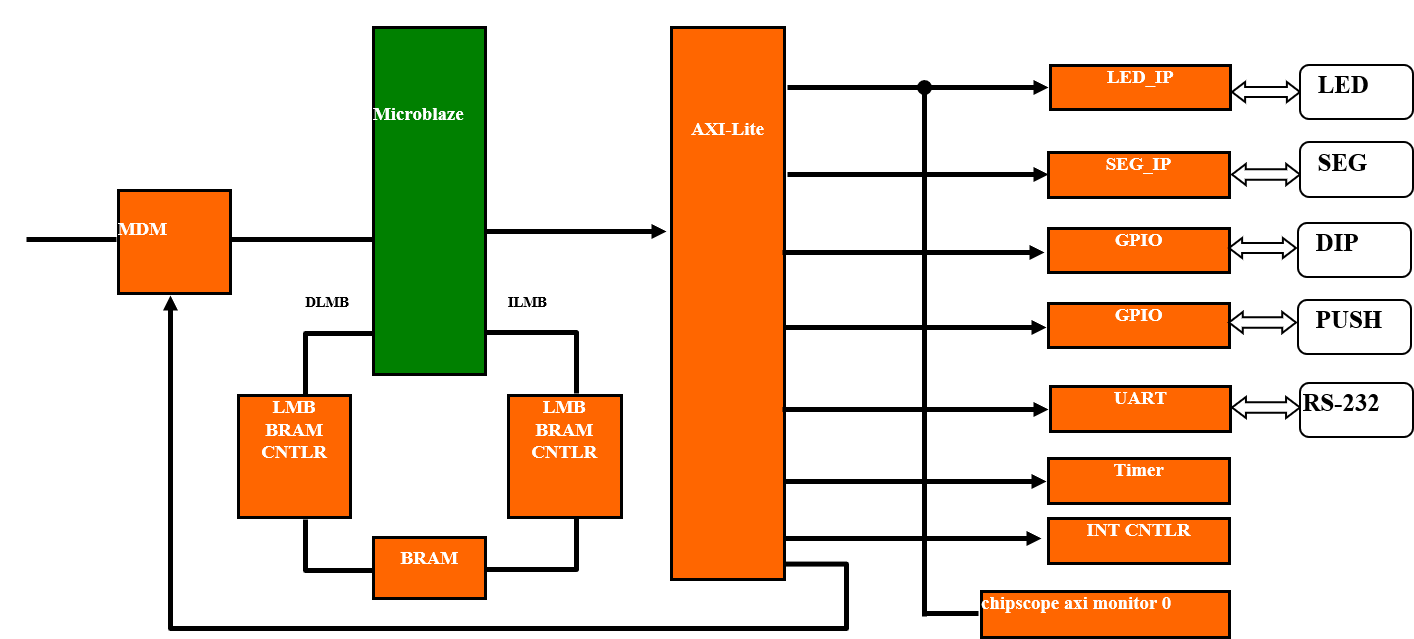
\includegraphics[width=1\linewidth]{report3-1}
  \caption{系统完整结构}
  \label{fig:report3-1}
\end{figure}

\begin{figure}
\centering
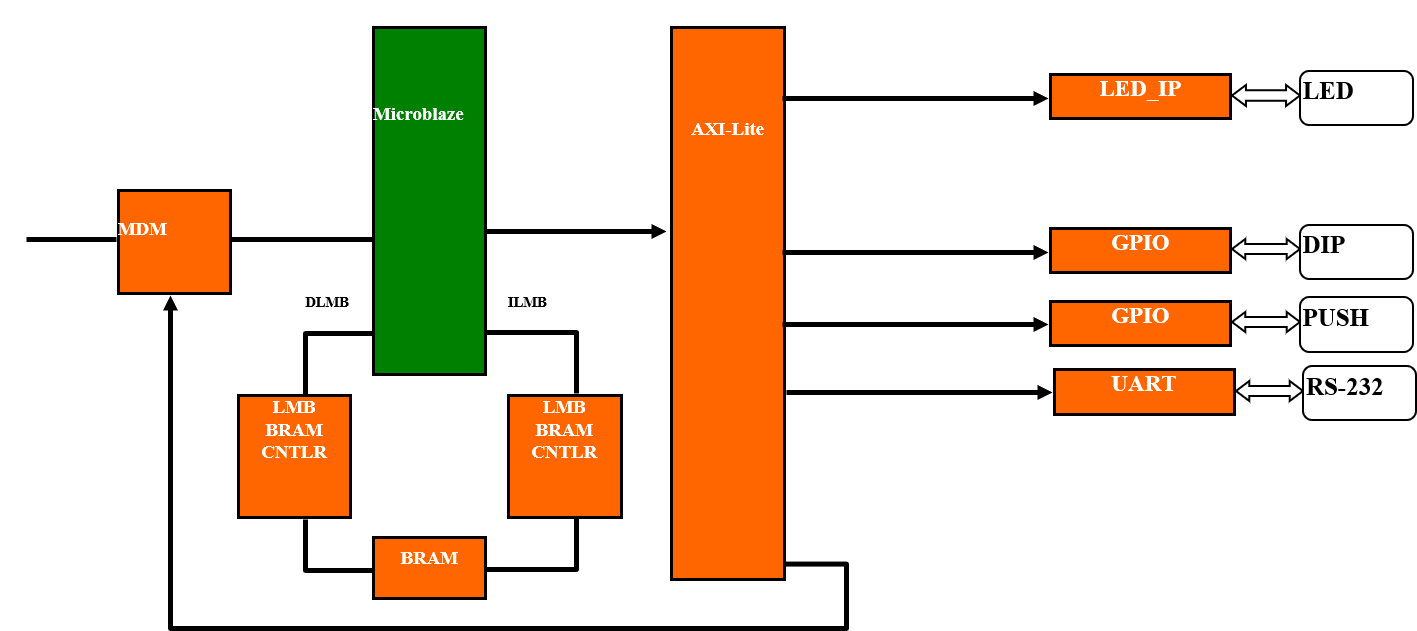
\includegraphics[width=1\linewidth]{report4-1}
\caption{本次试验的系统内容}
\label{fig:report4-1}
\end{figure}

\subsubsection{自定义 IP 核}

将之前的实验的内容复制一份新的出来,并在 XPS 中打开。

在 \verb|Hardware -> Create or Import Peripheral| 中创建一个新的外设。

在向导中选择 创建新外设的模版。
然后并在其中导入 XPS 工程。将 IP 核的名字命名为 \verb|led_ip| 。

其中总线的类型选择 \verb|AXI_Lite|,并且将 \verb|IPIF (IP Interface) Services| 配置项中的 \verb|Include data phase timer| 取消选中的状态。然后配置寄存器的个数为 $1$ 。

其余的内容基本保持默认,然后在\verb|(OPTIONAL) Peripheral Implementation Support| 中选择生成 ISE 工程与外设驱动模版。

最后点击 \verb|Finish| 完成配置。

\subsubsection{自定义 IP 核逻辑}

在 XPS 中双击 IP 核添加到设计中,可以保持默认设置,由 XPS 自动进行连接总线。

在 \verb|Bus Interface| 中选择创建的 IP 核 的实例,然后分别编辑处理器外设描述文件,与 IP 核的 HDL 源代码。

\paragraph{处理器外设配置文件}

在 文件大概 38行位置,有着\lstinline[language=bash]|## Ports| 这一行注释的下面编辑内容添加端口:
\begin{lstlisting}
PORT LED = "", DIR = O, VEC = [7:0]
\end{lstlisting}

\paragraph{编辑 user\_logic.vhd 文件}

在大约 100 行处,添加用户自定义端口的地方添加端口声明:
\begin{lstlisting}[language=VHDL]
led : out STD_LOGIC_VECTOR( 7 downto 0);
\end{lstlisting}

并在大约 147 行的位置处,添加将寄存器赋给led关口的代码:
\begin{lstlisting}[language=VHDL]
led <= slv_reg0(7 downto 0);
\end{lstlisting}

\paragraph{编辑 led\_ip.vhd 文件}

然后在141 行处添加对 led 的端口:
\begin{lstlisting}[language=VHDL]
led : out STD_LOGIC_VECTOR(7 downto 0);
\end{lstlisting}

然后在 大约 306 处添加对端口的映射:
\begin{lstlisting}[language=VHDL]
led => led,
\end{lstlisting}

\subsubsection{连接 IP 核}

然后选择 \verb|Project -> Rescan User Repositories| 刷新仓库,使
更改生效。
在 Ports 标签下,将 led\_ip 的led端口设为外部端口。

然后打开系统的用户约束文件\verb|system.ucf| 为期添加脚针的用户约束:
\begin{lstlisting}
#
# pin constraints
#
NET GCLK LOC = "V10"  |  IOSTANDARD = "LVCMOS33";
NET RESET LOC = "B8"  |  IOSTANDARD = "LVCMOS33"  |  TIG;
NET RS232_Uart_1_sin LOC = "N17"  |  IOSTANDARD = "LVCMOS33";
NET RS232_Uart_1_sout LOC = "N18"  |  IOSTANDARD = "LVCMOS33";
#
# additional constraints
#

NET "GCLK" TNM_NET = sys_clk_pin;
TIMESPEC TS_sys_clk_pin = PERIOD sys_clk_pin 100000 kHz;

## Switches
Net "dip_GPIO_IO_I_pin<0>" LOC = T10 | IOSTANDARD = LVCMOS33;
Net "dip_GPIO_IO_I_pin<1>" LOC = T9 | IOSTANDARD = LVCMOS33;
Net "dip_GPIO_IO_I_pin<2>" LOC = V9 | IOSTANDARD = LVCMOS33;
Net "dip_GPIO_IO_I_pin<3>" LOC = M8 | IOSTANDARD = LVCMOS33;
Net "dip_GPIO_IO_I_pin<4>" LOC = N8 | IOSTANDARD = LVCMOS33;
Net "dip_GPIO_IO_I_pin<5>" LOC = U8 | IOSTANDARD = LVCMOS33;
Net "dip_GPIO_IO_I_pin<6>" LOC = V8 | IOSTANDARD = LVCMOS33;
Net "dip_GPIO_IO_I_pin<7>" LOC = T5 | IOSTANDARD = LVCMOS33;

## Buttons
Net "push_GPIO_IO_I_pin<0>" LOC = A8 | IOSTANDARD = LVCMOS33;
Net "push_GPIO_IO_I_pin<1>" LOC = C4 | IOSTANDARD = LVCMOS33;
Net "push_GPIO_IO_I_pin<2>" LOC = C9 | IOSTANDARD = LVCMOS33;
Net "push_GPIO_IO_I_pin<3>" LOC = D9 | IOSTANDARD = LVCMOS33;

## Leds
Net "led_ip_0_LED_pin<0>" LOC = U16 | IOSTANDARD = LVCMOS33; 
Net "led_ip_0_LED_pin<1>" LOC = V16 |  IOSTANDARD = LVCMOS33; 
Net "led_ip_0_LED_pin<2>" LOC = U15 |  IOSTANDARD = LVCMOS33; 
Net "led_ip_0_LED_pin<3>" LOC = V15 |  IOSTANDARD = LVCMOS33; 
Net "led_ip_0_LED_pin<4>" LOC = M11 |  IOSTANDARD = LVCMOS33; 
Net "led_ip_0_LED_pin<5>" LOC = N11 |  IOSTANDARD = LVCMOS33;
Net "led_ip_0_LED_pin<6>" LOC = R11 |  IOSTANDARD = LVCMOS33; 
Net "led_ip_0_LED_pin<7>" LOC = T11 |  IOSTANDARD = LVCMOS33;
\end{lstlisting}

\subsubsection{生成网表与比特流}

在 XPS 中生成 网表与比特流。

\subsubsection{生成软件工程}

选择 \verb|Project -> Export Hardware Design to SDK| 然后导出并启动 SDK。
然后将工作空间定位到 \verb|SDK\SDK_Export\| 下。并删除之前的两个工程(与磁盘文件)。

然后按照之前的实验中的步骤,重新生成新的板级支持包。
然后在为之创建一个新的空白工程。

然后在 SDK 中的 \verb|Xilinx Tools -> Repositories| 中添加当前目录,然后刷新从新扫描。

之后修改板级支持包,重新配置 led 的 IP 核。

然后修改 \verb|drivers\led_ip_v1_00_a\src| 下的 \verb|led_ip_selftest.c| 文件下添加一行代码:
\begin{lstlisting}[language=C]
#define LED_IP_USER_NUM_REG 0x1
\end{lstlisting}

然后为创建的空的项目导入 资料中的 lab3.c 文件中的代码,然后编译真个工程。



\subsubsection{上板上电}

在代码保存之后,程序是自动编译的,因此至此所需要的文件基本都准备好了。
        
        \paragraph{链接串口}
        
        在之前设计硬件的部分是使用串口进行通信。在 Windows 上使用
        PuTTY这个软件进行与 FPGA 开发板的通行。对于 macOS 或者 Linux
        等 Unix类的系统则是使用 minicon 进行串口的链接。
        
        之前配置的是 波特率是 115200,则在配置中配置好。
        
        然后在JTAG 配置中,配置成 Diligent 的 USB。然后将之前生成好的文件通过
        \verb|Xilinx Tools -> Program FPGA|  中的选项配置好的比特流文件与生成的可执行的ELF文件,将其刷入 FPGA中。

        然后在串口链接工具中可以看见输出的内容。




\end{document}